\documentclass{beamer}
%\usepackage{split}

\usepackage{amsmath}
\usepackage{amsfonts}
\usepackage{braket}
\usepackage{subcaption}
\usepackage{tikz}
\usepackage{xcolor}
\usepackage{svg}
\usetikzlibrary{positioning,shapes,arrows.meta}
%\usetikzlibrary{positioning,fit,backgrounds}
\usepackage{quantikz}
\usepackage[linesnumbered]{algorithm2e}
\usepackage{hyperref}
%\usepackage{hyperref,xcolor}
%\usepackage[ocgcolorlinks]{ocgx2}
\usepackage{cleveref}
\usepackage[backend=biber,style=alphabetic,sorting=ynt]{biblatex}
\addbibresource{./sample.bib}


\input{newcommands}


\newcommand*{\QACze}{ \mathbf{QAC}_{0} }
\newcommand*{\QNCzef}{ \mathbf{QNC}_{0,f} }
\newcommand*{\QNCze}{ \mathbf{QNC}_{0} }
\newcommand*{\QNCon}{ \mathbf{QNC}_{1} }
\newcommand*{\NCon}{ \mathbf{NC}_{1} }
\newcommand*{\noiseQNCon}{ noisy-$\QNCon$ }
\newcommand*{\QNC}{ \mathbf{QNC} }
\newcommand*{\QNCG}{ \mathbf{QNC_G} }
\newcommand*{\NC}{\mathbf{NC}}
\newcommand*{\QNCiG}{\mathbf{QNC_{G,i}}}



\usetikzlibrary{patterns, shapes.arrows}
\usepackage{tkz-graph}
\usetikzlibrary{decorations.pathmorphing}
\usepackage{tkz-berge}

\usetikzlibrary{intersections}

\usepackage{cancel}
\begin{document} 

%\newcommand*{\Tr}{\textbf{Tr }}


\begin{frame}
  \title{Topological Memory - Dependence}
    \author{David Ponarovsky}
    \date{\today}
    \titlepage
\end{frame}


\begin{frame}

\frametitle{Introduction}
\begin{block}{Today:}
\begin{itemize}
  \item Dependence. 
  \item Local Stochastic Noise.  
\end{itemize}
\end{block}
\end{frame}

% ------------------------------------------------ $ 
  


\begin{frame}
  \frametitle{Dependence Type I}
  \begin{figure}[h]
    \begin{tikzpicture}[scale=0.7]
      %\draw node at (1.5,4.5) {$v_{2}$ is flipped.};

\draw node (u1) at (3,3) [draw,shape=rectangle]{$u_1$};
\draw node (x) at (0,6) [draw,shape=circle]{$x$};
\draw node (y) at (0,0) [draw,shape=circle]{$y$};
\draw (u1) -- (y)
  (u1) -- (x);
\end{tikzpicture}
  \end{figure}

  \begin{align*}
    & \prb{ (x,y) \in e | u_{1} \text{ is satisfied} }  \\
    & = \prb{ x \in e | u_{1} \text{ is satisfied}  }  \prb{ y \in e | u_{1} \text{ is satisfied}  } \\ 
    & \le \prb{ x \in e }\prb{ y \in e }
  \end{align*}

\end{frame}

\begin{frame}
  \frametitle{Dependence Type II}
  \begin{figure}[h]
    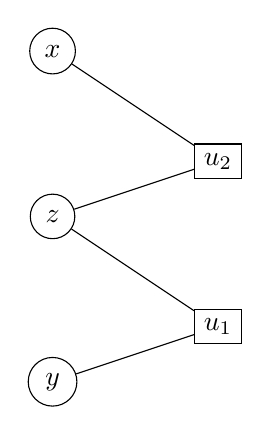
\begin{tikzpicture}[scale=0.7]
      %\draw node at (1.5,4.5) {$v_{2}$ is flipped.};

\draw node (u1) at (3,1) [draw,shape=rectangle]{$u_1$};
\draw node(u2) at (3,4) [draw,shape=rectangle]{$u_2$};
\draw node (x) at (0,6) [draw,shape=circle]{$x$};
\draw node (z) at (0,3) [draw,shape=circle]{$z$};
\draw node (y) at (0,0) [draw,shape=circle]{$y$};
\draw (u1) -- (y)
  (u1) -- (z)
  (u2) -- (x)
  (u2) -- (z);
\end{tikzpicture}
  \end{figure}

  \begin{align*}
    & \prb{ (x,y) \in e | z \text{ is not flipped} }  \\
    & = \prb{ x \in e | z \text{ is not flipped} }  \prb{ y \in e | z \text{ is not flipped} } \\ 
    & \le \prb{ x \in e }\prb{ y \in e }
  \end{align*}

\end{frame}


\begin{frame}
  \begin{block}{Definition}
Consider two (qu)bits $x,y$. We say that $z$ is a \textbf{linked node} between $x$ and $y$ if $z$ is either a bit or a check that is shared by both of their $D$ light cones.
  \end{block}

  \begin{block}{Remark}
    Notice that $y$ might be a \textbf{linked node} between $x$ and $y$.
  \end{block}

  \begin{block}{Definition}
    Consider an application of a noise channel. We say that $z$ is a \textbf{clean linked node} if:
    \begin{enumerate}
      \item $z$ is a bit and  $z \notin f$ (not flipped). 
      \item $z$ is a check and $z$ is satisfied. 
    \end{enumerate}
  \end{block}
\end{frame}


\begin{frame}

  \begin{align*}
    &\prb{x_{1},x_{2}, .. x_{k}, x_{k+1}, .. x_{l} \in e | z_{1},z_{2},..z_{m} }  \\
    = & \prod_{i}\prb{x_{i} \in e | z_{1},z_{2},..z_{m} } \\ 
    = & \prod_{i}\prb{x_{i} \in e | z \in \Gamma(x_{i}) } \\ 
    \le & \prod_{i}^{k}\prb{x_{i} \in e} \prod_{i=k+1}^{l}\prb{x_{i} \in e | z_{i} \in \Gamma(x_{i}) } \\ 
    \le & M(p)^{k}  
  \end{align*}

\end{frame}



\begin{frame}
  \frametitle{McDiarmid's Inequality - Local Stochastic Noise}

  
  \begin{block}{$C_{1},C_{2}$- local stochastic noise}
    Let $C_{1}, C_{2} > 0$. We say that $\rho$ is subjected to $C_{1},C_{2}$- local stochastic noise, if for any subset of qubits $S$ the probability they will be faulty is bounded by:  
    \begin{align*}
      C_{1}p^{|S|} \le \prb{S \in e} \le C_{2}p^{|S|} 
    \end{align*}
  \end{block}
  

  \begin{block}{Lemma: McDiarmid's Inequality}
    McDiarmid's Inequality is correct for $C_{1},C_{2}$- local stochastic noise. 
  \end{block}

\end{frame}
\begin{frame}
  \frametitle{Proof}
  \begin{block}{Proof}
    Consider \href{https://people.eecs.berkeley.edu/~bartlett/courses/281b-sp06/bdddiff.pdf}{ref}. We have to bound:
    \begin{align*}
      \star = \sup_{x,\bar{x}}\expp{f|X_{1},..X_{i-1},x} - \expp{f|X_{1},..X_{i-1},\bar{x}}
\end{align*}

First we show that: 

    \begin{align*}
      & \frac{C_{2}}{C_{1}}p^{|Z|} & \le \prb{z_{i+1},..z_{n}|X_{1},..X_{i-1},x} & \le \frac{C_{2}}{C_{1}}p^{|Z|} \\ 
      & \frac{C_{2}}{C_{1}}p^{|Z|} & \le \prb{z_{i+1},..z_{n}|X_{1},..X_{i-1},\bar{x}} & \le \frac{C_{2}}{C_{1}}p^{|Z|} 
\end{align*}

\end{block}
\end{frame}
\begin{frame}
  \frametitle{Proof}

And then we get that: 

\begin{align*}
  \star & \le \sum_{Z}p^{|Z|}\left( \frac{C_{2}}{C_{1}} -  \frac{C_{1}}{C_{2}} \right) c \\
  & \le c\left( \frac{C_{2}}{C_{1}} -  \frac{C_{1}}{C_{2}} \right) \frac{1}{1 - p }
\end{align*}

\end{frame}


\begin{frame}
  \frametitle{Trick.}
Suppose that $\prb{S}$ is not bounded from beneath by $C_{1}p^{|S|}$. Then one can define the distribution $\mathcal{D}^{\prime}$ such that:
  \begin{align*}
    \mathcal{D}^{\prime}(S) = \begin{cases}
      \mathcal{D}(S) & \text{if }\mathcal{D}(S) > C_{1}p^{|S|} \\
      C_{1}p^{|S|} & \text{else} 
    \end{cases}
  \end{align*}
  
And notice that probabilities might sum up to more than $1$. Then: 
\begin{align*}
  & \prbm{f - \exppm{f}{ \sim\mathcal{D} } > t }{\sim\mathcal{D}} \le \prbm{f - \exppm{f}{ \sim\mathcal{D} } > t }{\sim\mathcal{D}^{\prime}} \\ 
  = & \prbm{f - \exppm{f}{ \sim\mathcal{D}^{\prime} } > t + \exppm{f}{ \sim\mathcal{D}^{\prime} } -  \exppm{f}{ \sim\mathcal{D} } }{\sim\mathcal{D}^{\prime}} \\ 
  \le &\prbm{f - \exppm{f}{ \sim\mathcal{D}^{\prime} } > \frac{t}{2} }{\sim\mathcal{D}^{\prime}} 
\end{align*}

 
\end{frame}





\begin{frame}
  \frametitle{Local Decoder} 
  
  \begin{block}{definition}
    We say that $D$ is a local decoder if when applied against $2p(1-p)$-depolarized channel: 
    \begin{itemize}
      \item  There exists function $M : (0,1) \rightarrow (0,1) $ such that the probability of each bit being flipped is $M(2p(1-p)) < p^{\frac{100}{99}}$.
      \item There is a constant $l$ such that for any bit, there are only $(\Delta)^{l}$ bits on which the event of it being flipped depends.
    \end{itemize}
For example, if we take $k$ large enough and consider the $(n,k)$-Toric, then both the swift-rule and the flip upon majority are local decoders.
  \end{block}
\end{frame}

\begin{frame}
  \begin{block}{Definition}
Consider the moment after the application of the depolarizing channel, and right before the correction by the decoder.

For a subset of qubits $S$, we say that a qubit $x \in S$ is depended if there exists $y \in S$ such:
\begin{enumerate}
  \item Either $x$ and $y$ share a check that is not satisfied. (Type I)  
  \item Or, $x$ and $y$ have checks which share a bit that was flipped by the application of the channel. (Type II)
\end{enumerate}
  \end{block}
\end{frame}


\end{document}
